%===================================== CHAP 2 =================================

\chapter{Background}\label{chpt:background}

% Connectionism
\section{Connectionism and Deep Learning}
The processing unit in an artificial neural network (ANN) is the artificial neuron. This unit may be represented as a single activation value, symbolising a neuron's internal state. In order to process information, vectors of activation values representing neuronal activation in a layer may be multiplied with matrices of weights, representing connections between neurons of different layers, i.e. synapses and synaptic connection strengths. This linear algebra operation propagates information throughout the network, and is commonly known as feed-forward in the classical domain of neural networks. In order to arrive at a weight configuration which lets a network perform a certain task, it may be trained using gradient-descent in weight-space \citep{Hinton1989}. A common implementation is by  back-propagating an error signal backwards through the network whilst attempting to minimize the signal by adjusting the weights accordingly. The error is usually a loss function such as the l2-norm (see the appendix in \ref{l2-norm}) of the difference between an acquired output and a target output, which may be thought of as the Euclidean distance in space. This technique of training a neural network; back-propagation, was largely popularized by \cite{Rumelhart1986}. Furthermore, \cite{Rumelhart1986} made the important choice of electing the logistic function, also known as the sigmoidal-function, as their candidate transfer function for propagating activation values through synapses in their experiments and models. That is, the sum of a neuron's input is run through the function, which has two important characteristics: \textbf{(1)} it puts a lower and upper bound on the values which a neuron may take, (-1, 1), and \textbf{(2)} it is continuous and differentiable, resulting in numeric methods of differentiation being applicable for weight adjustment relative to the change in activation values. In other words, the transfer function may be thought of as a crude mathemtical approximation to a neuron's internal dynamics.
When ANNs are constructed in this manner; as simple activation values, weights between the values, and transfer functions between the different layers, the resulting models are quite often referred to as connectionist models. An example includes the aforementioned traditional feed-forward back-propagation (FFBP) neural networks of \citep{Rumelhart1986}.

% Other connectionist research here? Do I need further examples? Keith only mentioned that I should include and example from computational neuroscience. I feel that I should include some more stuff that condenses the context which I would like to establish for the model that I am actually investigating.
When it comes to deep learning, it is primarily an engineering discipline in the sense that its models are more focused on creating applicable systems and solutions, rather than on explaining the biological systems from which they originate. I would like to emphasize that despite this, it is the synthesis of neuroscience, psychology, and computer science that has given rise to the field of artificial neural networks \citep{McCulloch1943} and its various sub-fields, and continues to be a main factor in advancing the field's applications. This is exemplified by the recent deep learning algorithms in which the biologically inspired long short-term memory (LSTM) unit \citep{Hochreiter1997}, and the even more recently proposed, and perhaps simpler, gated recurrent unit (GRU) \citep{Mnih2015}, has enabled deep networks to capture temporal dependencies in data sets - adding a fundamental and crucial richness to what correlations and structures that may be captured by this class of general learning algorithms; namely long-term temporal dependencies within data. 
While a unit such as the GRU does not necessarily demonstrate the workings of the biological brain, it does demonstrate that looking at aspects which the biological brain captures, and translating them into algorithmic principles or requirements, may significantly improve engineered solutions, having both computer scientific value and impact. In other words; attaining further knowledge within the domain of computational neuroscience may lead to algorithmic advances within deep learning, and vice versa. Had the GRU been discovered first, this could have led to the hypothesizing of recurrence being crucial to capturing temporal dependencies within neural functioning. Even though this is already a widely appreciated fact within neuroscience, the LSTM and GRU may still have an impact on the field of neuroscience, as we continue to discover why they enable algorithms to perform more sophisticated types of processing. While it is not the aim of this thesis to categorize algorithms as belonging to one branch or another within the associated fields of neural networks, it is my intent to outline connectionism and computational neuroscience in order to \textit{clarify} the synthesis of fields related to neural networks and AI, as well as to establish the context for the model which is studied in this thesis. A further review of computational models is included later in this chapter, after a foundational neuroscientific background has been visited.

% (A Connectionistic= Outline of Memory and Intelligence - See above; synthesis and review of further models later in chapter.
% See my paper from UCL?


% =================================================================================================
\section{Catastrophic Forgetting}

Catastrophic forgetting \citep{McCloskey1989, Ratcliff1990} is as outlined in the introduction (chapter \ref{chpt:intro}) forgetting of model parameters for a domain in which the model has previously been trained. This may occur to such an extent that the network performance is equal to that of random weight initialization.

\cite{McCloskey1989} were some of the first to analyse catastrophic interference, noting that it seemed inevitable during sequential learning in connectionist models. Furthermore, they found that the cause for interference is that the newest weight adjustments reflect the newest information more heavily. In other words, old information is by the nature of the sequential learning disrupted by the correlations currently being extracted by the current pattern. This remains a fundamental issue for algorithms employing sequential learning, by using algorithms such as back-propagation, or other gradient-descent algorithms. In fact, it remains a central issue for all network-based algorithms which in a sense do not perform equal weight-adjustments in parallel.

\cite{Ratcliff1990} studied forgetting in neural networks, and found similarly to McCloskey and Cohen that back-propagation networks are prone to catastrophic forgetting. Furthermore, he found that as more information is learnt by an FFBP ANN model, its ability to discriminate between previously presented patterns and the ones currently being learned is actually reduced. This contrasts empirical studies of biological neural networks \citep{Ratcliff1990}, and led \cite{Ratcliff1990} to propose a mechanism for reducing catastrophic forgetting in ANNs. Namely by using neurons which would selectively \textit{respond} to certain input, thus naming the neurons 'response nodes'. His proposed model did not successfully alleviate the problem of catastrophic forgetting, however. Note that various attempts were made by both of the two aforementioned authors, \citep{McCloskey1989, Ratcliff1990}, none of whom attained a model which would alleviate catastrophic forgetting in FFBP ANNs.
% French's node sharpening:
\cite{French1992} examined FFBP ANNs in a very similar context, attempting to alleviate catastrophic forgetting by implementing 'node sharpening'. Arguing that catastrophic interference occurs due to overlap in input patterns, \cite{French1992} suggested that the issue could be alleviated, or even resolved, by creating a non-overlapping memory. Therefore he reviewed previous research such as the ALCOVE algorithm \citep{Kruschke1992}, on using a sparse distributed memory, in which information would rarely overlap. He found this to alleviate catastrophic forgetting to a certain extent. However, it did so by implementing a very large address space. Once this address space would become digested, catastrophic forgetting would indeed still occur. It is worth noting that using a sparse distributed memory requires an algorithm to be able to construct hyperplanes in which the input data is successfully separated. This may result in less generalisability in the network model, if representations are distributed across distinct sub-networks due to the hyperplane mapping.
Node sharpening as proposed by \cite{French1992} locally constrains input patterns to enhance the most prominent input features, effectively resulting in sparse representations. This results in less "noise" being propagated throughout the network, the most principal input nodes being in focus, and a significant reduction in catastrophic forgetting. However, this is done at the cost of attaining a less generalisable model, as node sharpening only looks at the \textit{n} most prominent nodes. This is strikingly similar to using convolutional networks for feature extraction, which was one of the inventions that re-instated neural networks as the state-of-the-art within domains such as image classification \citep{LeCun2015}. It should be noted that today's solutions such as the seminal deep convolutional network of \cite{Krizhevsky2012} performs a much more rigorous analysis of the input vector before passing it along to the subsequent layers of the network. Additionally, the method with which node sharpening is performed is a fairly biologically implausible algorithm, though feature extraction itself, e.g. extracting the most important features within a visual scene, is believed to occur biologically speaking. The mechanism with which this occurs is believed to be more similar to feature extraction using ConvNets, the convolution operation, however, being performed by the plastic neural network itself.
Today's state-of-the-art algorithms do furthermore employ different transfer functions, network topologies, and neuron-models, when compared to French's (1992) node sharpening model. This may render his claim within the paper obsolete; namely that a trade-off between catastrophic forgetting and generalisation is inevitable.
Building on French's (1992) former work, \cite{French1994} proposes a model which \textit{dynamically} sharpens the most relevant input nodes. Once two different outputs have been presented to a standard FFBP network, a context bias is calculated in the hidden layer, and propagated back to the input layer. Shortly put, this emphasizes the differences of the distinct categories, focusing on segmenting and orthogonalizing on the most prominent properties of difference. Which results in more orthogonal, well distributed patterns being learned.
Although this type of segmentation works well, it is still very similar to the former approach of \cite{French1992}, and suffers from the same trade-off between remembering and generalisation. As in other FFBP networks performing gradient descent in weight space, the algorithm will only succeed to find the most principal components, scaling with how much information the network is able to store (mainly affected by its size). As a consequence, failing to attain a sufficient accuracy for a given task could be due to ignoring the detailed information present in the segmentation process. Furthermore, it may be the case that only finding the most principal correlations in a distribution does not reveal the distribution's true nature, failing to extract precise correlations and properties. This is at the very core of the sensitivity-stability dilemma \citep{Hebb1949}, i.e. the trade-off which occurs between the learning of new and disruption of old information. One way way of addressing this dilemma is by multi-network systems, which \cite{French1994} suggests in his conclusion. This may produce refined solutions and abstractions and more sophisticated pattern-associations, although seemingly less computationally efficient. In this thesis, the dual-network memory architecture \citep{McClelland1995} is the elected architecture for model construction and implementation, addressing catastrophic interference, and how short- and long-term memory may be implemented by the brain. The state-of-the-art of dual-network memory architectures is reviewed below in chapter \ref{chpt:existing-models}. Before this model is presented, required background material from neuroscience will be presented.


% -> Computational Neuroscience
\section{Computational Neuroscience}

At the other end of the scale of using neural networks to study emergent behaviour, we have computational neuroscience,  where the principle of Hebbian learning is often the elected learning mechanism, yielding a greater biological plausibility in the computational models in aspects such as that Hebbian learning converges very quickly (one-shot learning is also possible, and occurs in the model which is outlined in chapter \ref{chpt:existing-models}). Another aspect which may regarded as biologically plausible is the algorithm k-winners-takes-all (kWTA), where the plausiblity arises from regarding it as implementing lateral inhibition. In biological networks, lateral inhibition may occur due to inhibitory neurons suppressing the activation of other neurons \citep{Rolls1998chpt1}; thus the term long-term depression. As for kWTA; the k-winners may be regarded as inhibiting the neighbouring neurons of the layer. Note that the algorithmic approach diverges from the biological in that lateral inhibition may be arbitrary, and for a fixed number of k neurons. Furthermore, depending on the implementation, activation values may be fixed, and possibly binary.

%\subsection{Background}
While it is assumed that the reader is familiar with neural networks within AI, it is not assumed that the reader has any prior knowledge within neuroscience. Therefore I will present an overview of the neuroscientific concepts used in this thesis, with the aim of sufficiently covering the neuroscientific background.
\\

% The very basics
As touched upon in the introduction, AI and neural networks borrows quite a bit of its vocabulary from neuroscience. One is very likely to encounter terms such as synapses, axons and dendrites when consulting the literature in computational neuroscience and other related disciplines. These terms refer to the connections between neurons, and the branches which physically enable them, respectively. A synapse actually consists of an axon, also referred to as a neuronal terminal, and a dendrite. Action potential may be propagated through an axon and its synaptic cleft to its connected dendrites, whose small branches are stretched out from other neurons' somata, or cell bodies - lying very closely to an axon terminal, and thus being referred to as connected. When a neuron is intracellularly, i.e. internally, excited above a certain level, this triggers a response which results in the release of neurotransmitters, specific molecules, through its axon terminal. These neurotransmitters may then bind to the receptors, other molecular structures that bind to specific neurotransmitters, which are on the surface of the dendrite, triggering an intracellular response in the receiving neuron \citep{Campbell2010chpt9}. From this short outline of synaptic communication, it is possible to see how biological neuronal functioning potentially provides for a much richer type of information processing, when compared to the crude mathematical approximations that are used in most neural network models. I will, however, regard cognition through a connectionist lens. As argued by Hebb, the framework with which we study aspects of cognition has to be scientific. Therefore it has to be axiomatic, and deterministic in the sense of being algorithmically implementable. Furthermore, I argue that although approximations are made in artificial models, it may be possible to extract mechanisms, properties, and principles of biological neural network functioning. Upon extraction, these principles may be implemented and executed, studied, and perhaps even successful in capturing specific emergent aspects of cognition. Some examples of computational models which have been able to do so are spatial navigation in place fields and place cells \citep{OKeefe1976, OKeefe1996}, and the recently discovered grid cells \citep{Hafting2005}. I will get back to these computational models below, and outline how they are related to spatial navigation and memory in the entorhinal cortex and hippocampus. 
% Whether a mechanistic neuron-level understanding of the brain can be attained, and whether it encompasses what is required to have cognition emerge, remains another discussion. I would therefore like to emphasise that as long as proven otherwise, the scientific method has to be employed, a testable framework needs to be used, and we cannot but assume that aspects of cognition may be captured by a mechanistic neural level understanding of the brain.
% For a discussion on this topic, I would like to refer the reader to \citep{Berg2016}.

%\subsection{Computational Basis for Constructing Theories About Brain Function}
Propagation of action potentials may lead to synaptic modification in that dendritic branches grows more closely to certain axon branches and terminals, thus being more respondent to the preceding neuron's activity and release of neurotransmitters. This process, along with a neuron's activity may be simplified and modeled as an activation value and function for the internal neuronal dynamics, together with a weight symbolizing the synaptic connection strength. Various algorithms may be employed for synaptic weight modification in the computational model, as well as for adjusting neuronal activation values. These different approaches may be hybrids of three neural network types \citep{Rolls1998chpt1}; \textbf{(1)} conditioned stimulus with associatively modifiable synapses, i.e. Hebbian learning, or standard feed-forward back-propagation networks, \textbf{(2)} purely recurrently connected associative networks, also known as Hopfield networks \citep{Hopfield1982}, and \textbf{(3)} k-winners-takes-all architectures, in which lateral inhibition is algorithmically simulated through letting the k most active neurons fire, possibly with the remaining firing beneath a certain, low threshold. All of these approaches can be said to capture aspects of long-term potentiation in neural networks. However, the algorithm with which a network learns, i.e. how a network attains its weight-configuration, cannot be said to be biologically plausible in the case of minimizing an error signal through back-propagation. Hebbian learning, however, is more biologically realistic, as it updates its weights according to the firing activity between neurons, often representing firing rates. Interestingly, ANNs using Hebbian learning converges very quickly, which is not the case when using FFBP.

%\subsection{Hippocampus and Memory}

Nearly half a century ago, \cite{Marr1971} argued that the hippocampus acts as a type of short-term or working memory, \citep{Rolls1998chpt6}. This has influenced later work, such as \citep{McClelland1995}, in proposing models where the hippocampus functions as an intermediary storage. The reasons for why the hippocampus has been hypothesized to be so are multiple. One is that it is generally recognized that the hippocampus receives input from nearly every part of the brain, either directly or indirectly \citep{Rolls1998chpt1}, and so has the required input to integrate across different stimuli, or memories. Another is that the computational models of hippocampal operation, built upon the empirical data of its structure, i.e. topology and functioning, have been shown to have qualities that are well suited to perform four essential operations that are related to memory and cognition.

Firstly, being able to quickly form new memories due to Hebbian learning is a crucial aspect for processing and remembering what happens during temporally constrained events. Therefore a mechanism for rapid learning needs to be present. As Hebbian learning performs weight adjustments according to the current firing pattern, this provides for a quickly converging learning mechanism in artificial neural networks. It is worth mentioning that one-shot learning is also made possible using Hebbian learning. 
When it comes to the potential storage capacity for memories in the hippocampus, there is a fairly large body of evidence suggesting that the hippocampus most likely employs a distributed type of encoding, resulting in that the capacity of \textit{patterns} which it may store is exponential to the number of neurons in a layer
\footnote{\label{footnote:Rolls98Chapters}Rolls, E. T., \& Treves, A. 1998. 'The hippocampus and memory', In: \textit{Neural Networks and Brain Function}. Oxford, UK: Oxford University Press. Chapter 6. Pp. 95-135}. However, this does not imply that an exponential number of \textit{pattern associations} may be stored, i.e. an exponential number of different stimulus-response patterns, as this has been found to increase only linearly with the number of neurons in empirical studies$^{\ref{footnote:Rolls98Chapters}}$.

Secondly, integrating across memories by using an auto-associative network, which is thought to be constituted by the highly recurrent CA3-layer of the hippocampus, may in fact be part of what cognitively enables the brain to contextualize the self and the present.

Thirdly, very much related to the former point of being able to integrate across several sources due to the recurrent nature of CA3, a mechanism for implementing a form of episodic memory is essential in order to remember events, and to temporally associate different memories with one another. This is thought to be constituted by the CA3- and CA1 layers, where activity is both projected from the CA3 to CA1 through so-called Schaffer collaterals, and also recurrently propagated to CA3. In other words, the CA1 may then possibly temporally associate consecutive integrated memories that are relayed from CA3.

Fourthly, the hippocampus has been found to back-project its activity from CA1 to the EC \citep{Rolls1998chpt6}, and to the neocortex. The output from CA1 to neocortical areas may be hypothesised to perform a type of both recall, and memory consolidation. Recall in that the patterns may simply invoke activity given its output, and memory consolidation in that this activity, after having been processed by the hippocampus, may be stored in the neocortex. Addressing the latter, the neocortex has been found to perform significant LTP in its circuitry \citep{Rolls1998chpt6}. Such consolidation has also been hypothesized to occur primarily during sleep \citep{French2001} in which a type of chaotic recall from a hippocampal network could produce pseudo-patterns which may be learnt by the neocortex.
\\


% Outlined specifics of how the outlined hippocampal functions may be algorithmically attained and/or biologically occur AFTER presenting material on neural network computation in general?
It may now begin to become clear to the reader how certain aspects of hippocampal function may be algorithmically described, and thus how certain aspects of cognition may emerge from implemented models. Furthermore, these aspects may then be analyzed both from a connectionist perspective with regarsd to cognition, and also with regards to the information processing capabilities that the emerging phenomena gives or may give rise to. A short outline has now been presented on how hippocampal functionality is connected to psychology and neuroscience. I will proceed to connect these aspects to computational modeling and algorithmics below.

% When it comes to how the distributed type of encoding is implemented, the empirical evidence suggests that 

One of the key components in the hippocampal neural processing as outlined by \cite{Hattori2014} in his model, is using kWTA in the layer-wise processing. He notes that kWTA seems to enable a much more sophisticated type of pattern-separation than ordinary transfer functions. This matches the observations and findings as outlined by \cite{Rolls1998chpt4, Rolls1998chpt6}. Namely that k-winners-takes-all will reduce overlap in that only the k most prominent units/neurons will dominate/inhibit the other neurons in a layer, and furthermore enable a more powerful separation of overlapping inputs. It should be emphasised that while kWTA may resemble lateral inhibition, selecting a paramter \textit{k} quickly becomes biologically implausible. Therefore, computational models often rely on empirical studies of levels of activation within different brain regions in order to attain more realistic models. One example is the model which is outlined below, where \cite{Hattori2014}, building upon the work of \cite{Wakagi2008}, finds that selecting k such that the layer-wise firing rate in his hippocampal module corresponds to the biologically observed firing rates does significantly improve the model performance. Furthermore, kWTA does indeed select 'only' k winners, and thus active neurons within a layer. I would like to emphasise that this leads to a quicker convergence and faster learning within the network, because weight updates may be performed only by the nodes which are deemed relevant with regard to the current pattern. In a sense, less "noise" from the other neurons is present, and a more clear correlation and possibly pattern association is likely to be present for the network to extract.
Lastly, it is worth mentioning that while kWTA may reduce overlap and separate inputs, it will also tend to result in similar patterns activating the same set of neurons. Therefore, kWTA may also be regarded as preprocessing which will categorize patterns into categories of similar types, \citep{Rolls1998chpt1}.

Another key aspect of computation previously outlined and present in the hippocampus, is auto-association and associative memory. Auto-association such as in a Hopfield network (see figure [figure:Hopfield net.]), associates one pattern with another very much like in a traditional network, only that the next activations are fed back into the very same layer, resulting in a mechanism for pattern completion. I.e. for only partial information of a previously learned pattern, the values from the pattern will be propagated through previously learned weights, which in turn reflect the pattern association previously learned. This will most likely result in that the consecutive patterns will more closely resemble the learned target pattern in the pattern association. From this abstract outline of the process, the reader might hopefully get a gist of both how auto-association enables recall through association of similar events and memories, not the least storage of these memories, but also why only a certain amount of memories may be stored in short-term memories working on these principles. This has been demonstrated in cases where an auto-associative network is taught two patterns that are too correlated. In that case, a simple Hopfield network will fail to perform pattern-completion, as it will be stuck between the two basins of attractions that are formed by the two different patterns \citep{Rolls1998chpt3}. This may be thought of as completing parts of for instance a pattern representing a letter, say 'a' - once part of the letter has been presented to the network; if another letter which is too similar, such as 'b' has been taught to the network, chances are that the Hopfield network then will push the network state towards both the 'a' and 'b' states at the same time. This will then ultimately lead to a new attractor state in which none of the letters is correctly recalled. Instead, it is likely that a combination of the two will be the result, or a cyclic pattern which cycles through hybrids of the two letters.
In the general case, the possible state-space of an auto-associative network may be visualised as a 3-dimensional space of matter, where the current input represents a point which moves in the space relative to gravity which is exerted on it in the space. Curvature in the space is then formed by training the network, which will result in points which the network is trained on to curve downward - attracting the point once it is allowed to recurrently cycle throughout the space. Analogously, when such a point is created, its surroundings is necessarily also affected a bit by this spatial curvature, and will therefore curve, although slightly less, downward, giving a direction during traversal. From this analogy it may be seen that if two such points are created in each others neighbourhood, there will be a given distance between them when the curvature exerted by the creation of both will form a new basin in between. Additionally, if too many such points are created, the landscape may become impossible to traverse, or even pointing to one or very few basins - which may very well also be hybrids of previously learnt patterns, i.e. spuriously created patterns.
This brings us toward the importance of other qualities that are present in hippocampal models which largely removes these problems of redundancy and convergence in the CA3-layer.

While the classic XOR-problem is a matter of linear separability, solvable by the introduction of non-linear transfer functions in FFBP ANNs, the forming of spurious basins of attraction in auto-associative networks may be addressed by qualities which are introduced by the hippocampus, and more specifically largely by the dentate granule cells of the dentate gyrus (DG), which project to CA3, both receiving projections from the entorhinal cortex (EC).

\textbf{Notes from Rolls \& Treves:}


Hopfield nets:
Content addressable memory - with partial pattern
Graceful degradation
Perfect recall (P. 46)

Expansion encoding in DG for decorrelation of overlapping separate memories in CA3, enabling separate storage and recall. Marr (1969), Rosenblatt's original perceptron similar w/ pre-processor. (P. 41)

The DNMM of \cite{Hattori2014} seems like a competitive network, having sparsification through in-EC and kWTA, and to some extent orthogonalization from the DG-layer through expansion encoding, as well as neuronal turnover. (P. 54)

[CHPT. 4]
Principal cells biologically mostly excitatory; mutual inhibition implemented by inhibitory interneurons. (GABA)

Qualities of hippocampal model lets it acquire more patterns. However, functions as STM. Discuss: Are these qualities transferable to networks in general? Principles? What do the experiments demonstrate?

Example of emergent phenomena implemented quite algorithmically, i.e. not through mechanisms resembling the biological mechanisms, yet having approximately the same emergent behaviour/aspects: k-WTA for lateral inhibition.

Could embed Mexican hat functionality, i.e. topographic influence from closeness in weight updates.

Feature discovery and self-organization - kWTA.

Redundance reduction using kWTA.

Orthogonalization leads to improved classification and/or categorization.

Diluted connectivity?

PCA not bio. plausible. k-WTA plausible. However, similar, yet not same type of orthogonalization.

This slow memory consolidation to the "neocortical" network could potentially suggest methods for storing the maximum amount of information in a network, if it can train the network to work when detached from the hippocampal network. \cite{French2001} found consolidation speed to be of no importance when it comes to retroactive network interference.
\\
Furthermore; implications for neuro. Model mainly concerned with neuro. ? Comp. Sc. Parallels?
\\

Role of DG-cells: 
1. Sparsification, orthogonalization, etc.
2. Reduce overlap and separate overlapping inputs using kWTA - i.e. inhibitory interneurons.
3. Low contact through MF (DG-CA3); sparsification.
4. May be powerful, i.e. force new pattern during learning.
\citep{Rolls1998chpt6}
\\

Biological plausibility of \citep{McClelland1995} architecture. Learning direct CA3-output implausible - however, may be regarded as an approximation to the neocortical back-projections through which learning may occur, and also produce fairly stable neocortical patterns \citep{Rolls1998chpt6}. Thus, the model is a very crude approximation to brain function on that level, without episodic memory which would be implemented by associating various CA3-ouputs in a CA1-layer.

\section{The Dual-Network Memory Architecture and Existing Models}\label{chpt:existing-models}[Needs elaboration]

In their seminal paper, \cite{McClelland1995} propose a dual-network memory architecture in which the hippocampus is responsible for the consolidation of memories to the neocortex, with the neocortex storing semantic and episodic memory. The synthesis of recall from the deeper layers of the neocortex and representations in the working memory itself enables contexts to be distinguished or connected in the proposed model. The learning and consolidation to the neocortical module is essentially performed in an interleaved fashion; slowly potentiating and instantiating the memories from the hippocampal to the neocortical network. An approach closely resembling a bottom-up and top-down synthesis, where recall is combined with novel patterns. This raises the question of how such an interconnectedness is constituted both topologically speaking, as well as in terms of local information-processing. Furthermore, the question is whether principles from the environment of the neocortex and hippocampus need to be extracted and implemented to successfully have this functionality emerge in computational models, i.e. whether a synthesis of brain functionality constituted by additional parts would be crucial in regard to memory consolidation in the artificial model. For instance for the successful integration across memories. The proposed model of \citep{McClelland1995} suggests that the hippocampus and neocortex constitute the mechanisms for successful integration across memories, as well as keeping memories fairly intact. The specifics on how these mechanisms are constituted, however, remain obscure or undiscovered. This constitutes a core inspiration and foundation for an artificial neural network (ANN) model in this thesis. More specifically it lays out the foundation for investigating long-term memory and memory consolidation, by which I hope to attain more insight into mechanisms that enable generalisability and plasticity in ANN models.

The model of \cite{McClelland1995} largely ameliorates the problem of catastrophic forgetting in ANNs, outperforming other algorithms of the time by far. However, work on this model is fairly limited, and it is with the aim of further extending the architecture that I review implementations of it.

\cite{French1997} propose a series of experiments that address the sensitivity-stability dilemma \citep{Hebb1949}, demonstrating that a pseudo-recurrent network model performs significantly better than traditional feed-forwad back-propagate networks, mainly inspired by \cite{McClelland1995}. Different experiments are used to illuminate several aspects of the pseudo-recurrent network model. The key finding is that pseudo-recurrent networks using pseudopatterns perform significantly better in terms of less catastrophic forgetting, suggesting that the brain may perform a type of pseudopattern compression and storage of information, too. Another point worth noting is that the networks that are simulated are of a fairly small scale, making them generalisable only to a certain extent due to network capacity. This seems to have been largely ignored by the authors. Therefore it would be interesting to look at the implications of both increasing the complexity as well as the scale of the network, such as in the models of \citep{Hattori2010, Hattori2014}. Note that the semi-distributedness of this paper's model arises naturally from the pseudo-recurrent neural network, as opposed to in the former papers of \cite{French1992, French1994}. This may suggest that the mechanism, which acts as an auto-associative memory, may also act as a predictor. In addition to completing incomplete, partial or fuzzy memories and retrieving them, it might therefore also provide a mechanism to filling in a story, or even imagining a story, creating it on the go by using the pseudo-recurrent mechanisms. This could suggest that the interleaving of memories in a pseudo-recurrent manner is at the heart of creativity, prediction and not the least; cognition. In relation to the thesis, I wish to investigate various successful or partly successful approaches for addressing convergence in the dual-network memory architecture. A key finding is that of pseudo-recurrence performing a crucial mechanism in interleaving and pattern generation. This may form a foundation for a comparative analysis in my future work, as well as providing insights into some underlying principles for the emergence of such mechanisms.

\cite{French2001} address the issues of the dual-network memory models in \citep{French1997, Ans1997}, illuminating key issues related to episodic memory, contextualisation, and pseudopattern generation and optimisation. In doing this, they conclude that the brain is likely to perform some kind of pseudopattern optimisation. Possibly in a stochastic way relative to how well it evaluates its performance and understanding of a currently perceived concept or state. When it comes to episodic memory, the work of \cite{Ans2000} is elaborated on, in which only dissimilar pseudo-inputs were used for consolidation to a neocortical network. Results demonstrated that the model was capable of generalising to and thus learning all patterns (20 patterns, where only 13 were explicitly taught to the neocortical network). This strengthens the view that a dual-network memory model is crucial for successful integration across memories. Another aspect that is addressed is contextualisation in the dual-network memory architecture. \cite{Ans2000} demonstrated that their implementation of a dual-network memory model performed better with pseudopatterns with random initial input rather than when retrieving similar patterns from the neocortical module. This does pose an inconsistency both biologically and algorithmically speaking, because it is biologically implausible to retrieve an output representing the activity of the entire neocortical network, and algorithmically inefficient or possibly intractable with increasing network size, in order to interleave new memories with old. Furthermore, retrieving similar patterns mostly leads to a failure of convergence. This suggests that there may in fact be other, or more, principles that play a crucial role in the dual-network memory architecture. Summarising; the dual-network memory model offers significant benefits and advances in neural network models, but there seems to be an oversimplification related to pseudopattern formation and generation, affecting the integration across similar, yet separate memories. This is an aspect which I wish to further investigate in this thesis.

\cite{Hattori2010} proposes a model which fundamentally differs from the former implementations of \cite{French1997, French2001}, and \cite{Ans1997} in that the hippocampal module is constituted by a chaotic neural network. Keep in mind that the phrases of hippocampal and neocortical networks should only be considered as borrowed terms for symbolising the networks of the model. The model networks are only very loosely coupled to biological functioning, with the approach outlined being only inspired by it.
\cite{Hattori2014} presents a novel ANN model based on his former work on the dual-memory architecture, where the short-term memory network is now a more complex and biologically plausible network; namely a simplified hippocampus model. \cite{Hattori2014} demonstrates in several experiments that catastrophic forgetting is reduced to a large extent in the new model, and furthermore that it is superior to the dual-network memory models of \cite{Ans1997, French1997, Hattori2010}. \cite{Hattori2014} further demonstrates that the hippocampal network is capable of acquiring information rapidly, consolidating this to the neocortical network when it is successfully extracted in the HPC module.
However, the model is still not used to solve complex tasks, as the model is rather heavy in terms of computational complexity due to introducing more complex neuronal dynamics. The hippocampal network consists of McCulloch \& Pitts neurons, using the Oja rule for learning and updating connections between the different sub-modules, and less contrained Hebbian learning with forgetting in the recurrent CA3-connections. Please see below for further details on the model.
As for his experiments and results, he finds that mean goodness and perfect recall is worse in the hetero-associative case when compared to the auto-associative for the model. This may suggest that a significant amount of plasticity is missing in the model. This is further supported by the observation that a much higher turnover-rate than observed biologically speaking has to be employed for tuning the model. Looking to complex systems theory, some noise or chaos is required to arrive at a phase-transition between regular and chaotic dynamics, i.e. the critical phase, in which learning is made possible and efficient, \cite{Langton1990, Newman2003}. By using a very high neuronal turnover in the model, this suggests that the high turnover rate could be what alleviates the lack of plasticity in the proposed model. Despite improving training performance and pattern extraction, using too high a turnover-rate may also introduce too much randomness, rendering the representations too coarse-grained. Therefore it would be interesting to see parameter adjustments for the hetero-associative case in the hippocampal module, as this may pose different constraints on the network. Particularly an analysis of the edge of chaos for the CA3-part is something which I wish to further investigate in my future work. Another important aspect would be attempting to temporally extend the model, in an attempt to capture how episodic memory may be constituted in a complementary memory model. Such a synthesis could potentially introduce novel aspects of high-level cognition. It is therefore my aim in this thesis to look at variations in neuronal dynamics as well as topologies in a novel dual-network memory architecture, first by introducing a novel neocortical network.

%\subsection{State-of-the-art}

\cite{Ans1997} demonstrated the important and interesting aspect of being able to increase a traditional FFBP ANN's storage capacity through embedding a learning algorithm using pseudo-patterns in a dual-network architecture. More recently, \cite{Hattori2010, Hattori2014} demonstrates that a dual-network memory model which is more biologically plausible may in fact extract patterns in a more effective and biologically resemblant way; nearly one-shot learning in an intermediary storage network. Thus having several qualities of short-term memory. Furthermore, his dual-network memory models show promising results in that they both outperform previous models of the architecture such as the models of \citep{French1997, Ans1997}, in classic sequential learning experiments for retroactive interference \citep{McCloskey1989}, where stimulus-response pairs of different training bases are learnt.
Hattori's (2014) model is reviewed and outlined below, which I present an algorithmic implementation and model of in chapter 3, followed by a chapter with experiments and results in chapter 4.

\subsubsection{The Neocortical Module}

\cite{Hattori2010} trains the neocortical module using pseudopatterns. A pseudopattern is a pattern representing the weighting and internal dynamics of a network. In his paper, \cite{Hattori2010} looks at two types of pseudopatterns, which he refers to as type I and II. Type I is constructed in a very simple way: A random input is presented to the neocortical network, and the output is retrieved. This is then stored as an input-output pattern, called a pseudopattern of type I.

Pseudopatterns of type II are constructed in a slightly different manner, the approach being as follows:

\begin{enumerate}
\item Retrieve an extracted pattern from the hippocampal network.
\item For each element of the pattern, reverse is with a probability $p_r$.
\item Present the pattern to the neocortical network, and store the retrieved input-output pair (pseudopattern II) in a set.
\item Repeat step 2. and 3. until a certain number of pseudopatterns of type II are obtained.
\end{enumerate}
Performing steps 1.-4. above results in a set of pseudopatterns of type II.

After pseudopatterns have been obtained, the neocortical network is simply trained on them by using FFBP, i.e. standard gradient-descent in weight space as outlined in \ref{BP}. Note that due to the nature of the pseudopatterns, old memories are actually interleaved with old. This may be seen by considering that pseudopattern I is in fact the output obtained by presenting a random input to the network, the output reflecting a compressed version of the network weights at the time. When the network is trained on the pseudopattern along with a hippocampal pseudopattern, BP attempts to minimise the error between the old configuration of weights and the new hippocampal pseudopattern. Thus interleaving the old representation of memories with the new memory. In fact, \cite{Hattori2014} uses the exact same type of mechanisms for memory consolidation to the neocortical network.
Similarly, for a set of pseudopatterns II, as elements are reversed in the hippocampal pseudopattern, the resulting pseudopatterns II reflect both the network configuration (weights) and the novel hippocampal pseudopattern. This is a more explicit type of interleaving, where a new pattern which is to be learned is slightly randomized, creating a set of patterns which will reflect both the new memory as well as the old.

Memory recall in the neocortical network may be performed by presenting input patterns to the neocortical network and obtaining the resulting output from the network. Note that as outlined above, the neocortical network only learns the pseudopatterns that are extracted by the hippocampal network. Therefore, some success criteria such as perfect recall depends strongly on the perfect extraction rate of the hippocampal network (i.e. when every part of the pattern has been successfully learned).

% ====================================
\subsubsection{The Hippocampal Module}
\subsubsection{\cite{Hattori2010}}
\begin{figure}
\centering
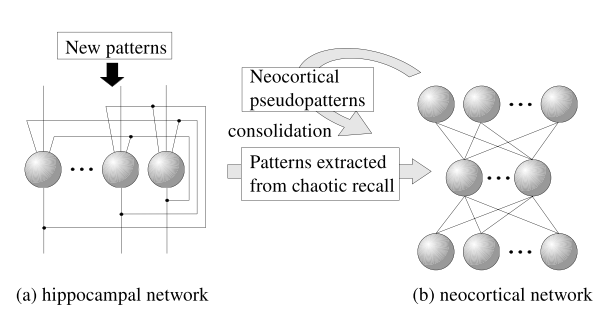
\includegraphics[width=10cm]{fig/hattori2010_model_structure}
\caption{(a) represents the hippocampal module, whereas (b) represents the neocortical module. Note that the hippocampal module implements a Hopfield network, from which seemingly chaotic behaviour emerges when combined with the neuronal dynamics. Adapted from Hattori, M. (2014). 'A biologically inspired dual-network memory model for reduction of catastrophic forgetting', \textit{Neurocomputing}, \textbf{134}: 262-268. Adapted with permission.}
\label{fig:hattori2010_model_structure}
\end{figure}

As can be seen from figure \ref{fig:hattori2010_model_structure}, \cite{Hattori2010} proposes a model in which the hippocampal (HPC) module is a single layer Hopfield network. However, the HPC module is not trained using gradient descent, but rather by Hebbian learning, which may be summarised as; fire together, wire together. Using Hebbian learning leads to faster convergence when compared to SGD \citep{Hattori2010}. Adopting \citeauthor{Hattori2010}'s (\citeyear{Hattori2010}) notation, the model may be formally outlined as follows, beginning with the equation for Hebbian learning;

\begin{equation}\label{hattori_hebbian_learning}
    \omega_{i,j}(t+1) = \gamma \omega_{i,j}(t) + x_i^{(k)} x_j^{(k)},
\end{equation}

where $\omega_{i,j}(t+1)$ is the weight between neurons $i$ and $j$ for time step $t+1$, $\gamma$ is a constant forgetting factor, $\gamma \in (0, 1)$, and $\textbf{x}^{(k)} = (x_1^{(k)}, x_2^{(k)}, ..., x_N^{(k)})$ is the $k$-th pattern that we want the network to learn. Note that $\textbf{x}^{(k)} \in \{-1,1\}^N$, which constrains $x_i^{(k)} x_j^{(k)} \in [-1,1] \implies \omega_{i,j} \in [-1-\gamma, 1+\gamma]$. $N$ is the number of nodes in the input patterns.

Further, \cite{Hattori2010} outlines the neuronal dynamics as follows;

\begin{equation}\label{hattori_next_output}
    u_j(t+1) = f\{\eta_j (t+1) + \zeta_j(t+1)\}
\end{equation}

\begin{equation}\label{hattori_former_inputs}
    \eta_j(t+1) = k_m \eta_j(t) + \sum_{i=1}^{N} \omega_{i,j} u_i(t)
\end{equation}

\begin{equation}\label{hattori_zeta}
    \zeta_j(t+1) = k_r \zeta_j(t) - \alpha u_j(t) + a_j
\end{equation}

Adopted to the thesis notation, $u_j$ is neuron $j$'s activation value, where the value for the next time step is determined by two functions, namely $\eta(t+1)$ and $\zeta(t+1)$. Equation \ref{hattori_former_inputs} takes into account its former input values through $\eta_j(t)$ for the current time step, in addition to summing over the inputs of its incoming synaptic connections. Equation \ref{hattori_zeta} includes a relationship to the neurons' previous activation values. Note that an external input parameter $a_j$ is also included in $\zeta_j(t+1)$, and that both equations \ref{hattori_former_inputs} and \ref{hattori_zeta} have damping factors of refractoriness $k_m$ and $k_r$, respectively, discontinuing the impact of former function-values exponentially relative to the temporal difference. $f(u)$ is the sigmoid function as defined in equation \ref{sigmoid}, note however that a steepness parameter $\epsilon$ is also included, $\theta$ being divided by $\epsilon$ such that,

\begin{center}
\begin{math}
    f(\theta) = \frac{1}{1 + e^{\frac{-\theta}{\epsilon}}}
\end{math}
\end{center}

% ====================================
\subsubsection{\cite{Hattori2014}}
\cite{Hattori2014} proposes a more biologically inspired dual-network memory model, based on and outperforming the model outlined above based on several experiments. In the novel model, \cite{Hattori2014} proposes a rather drastic architectural change in the hippocampal network, the neocortical module remaining the same. The hippocampal module is made out of five layers, the three middle layers being inspired by different parts of the hippocampus; namely the entorhinal cortex (EC), dentate gyrus (DG), and CA3, the first and last layer being the input and output layers. See figure \ref{fig:hattori_2014_model} for the topological structure of the novel model of \cite{Hattori2014}.

\begin{figure}
\centering
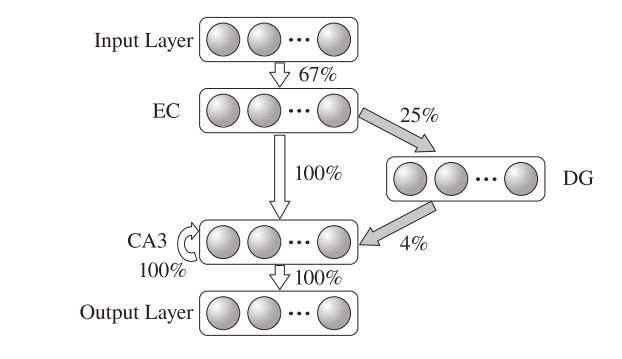
\includegraphics[width=10cm]{fig/hattori2014_hpc_module}
\caption{This figure illustrates Hattori's (2014) proposed dual-network memory model. Note that the EC is connected to both CA3 and DG, which in turn is also connected to CA3. The gray arrows are connections which are only used during training. Furthermore, CA3 is fully connected both recurrently as well as to the output layer. As EC is connected somewhat sparsely to the DG, and DG is very sparsely connected to CA3, this may constitute a form of compression mechanism as seen in auto-encoders. It is also worth noting that this poses a time-delay from when a certain input has been directly presented from the EC to CA3 until the possibly compressed input arrives from the DG. This may further constitute mechanisms similar to those of operating at multiple timescales, as well as mechanisms for abstraction.
Hattori, M. (2014). 'A biologically inspired dual-network memory model for reduction of catastrophic forgetting', \textit{Neurocomputing}, \textbf{134}: 262-268. Adapted with permission.}
\label{fig:hattori_2014_model}
\end{figure}

It is worth mentioning that a slightly different transfer function is used by \cite{Hattori2014}. Namely,

\begin{center}
    $f(\theta) = tanh(\frac{\theta}{\epsilon})$,
\end{center}
where $\epsilon$ still is a steepness parameter.

Hebbian learning is still used as in equation \ref{hattori_hebbian_learning} for the CA3-layer and the CA3 to output-layer, relative to its former output;

\begin{center}
\begin{math}
    \omega_{i,j}(t+1) = \gamma \omega_{i,j}(t) + u_i u_j
\end{math}
\end{center}

However, between the EC and DG, EC and CA3, and DG and CA3 parts, Oja's rule is used (\cite{Hertz1991}, cited in \cite{Hattori2014}). Oja's learning rule is a modified type of Hebbian learning, restricting the weight space (to prevent divergence as a result of the chaotic behaviour). It may be formally outlined as follows,

\begin{equation}\label{ojas_rule}
    \omega_{i,j} = \omega_{i,j}(t) + \lambda u_j (u_i - u_j \omega_{i,j}(t)),
\end{equation}
where $\lambda$ is the learning rate for the Oja neurons. Note that the input and output layer neurons are bipolar ($\pm 1$), whereas the other neurons are binary. Every region is trained by a k-winners-take-all (kWTA) approach, in which a fixed number of the $k$ most active neurons' activation values are propagated throughout the neurons' synapses. Neuronal activity is determined by firing frequency. Interestingly, \citep{Hattori2014} notes that the non-linear separation of kWTA seems to be far more powerful than that of non-linear transfer functions. Furthermore, he notes that non-linear transfer functions may actually reduce the performance of kWTA.

One of the final keys to attaining a successful dual-network memory model introduced by \cite{Hattori2014} is neuronal turnover. Neuronal turnover is the birth and extinction of a percentage $\beta \%$ of the neurons, here in the DG. Note, however, that while this is believed to occur to a very low degree biologically in the DG, a very high rate of $\beta = 50 \%$ is employed by \cite{Hattori2014}, with turnover after every training set. Possible reasons for this and associated implications, related to plasticity and convergence, is discussed earlier in this section. \cite{Hattori2014} further demonstrates that the input patterns become less similar when introducing the neuronal turnover, which in turn drastically increases the number of patterns that may be stored in the HPC module.

Memory recall may be performed in the hippocampal network by chaotic recall after learning, i.e. presenting random input to the different sub-networks, waiting until it reaches some convergence criterion, considering the current pattern as a recalled memory. Another approach for interleaving new memories with old, as proposed by \cite{French1997}, is by re-instantiating the previously learned patterns from the neocortical module to the hippocampal network, thus interleaving everything contained in the neocortical network with a new hippocampal pattern. While biologically implausible and not that relevant for the current approach as outlined here, it is worth noting that a similar mechanism for re-instantiated a previously learned pattern to the hippocampal network if present in the neocortical network, might result in attaining novel abstract representations. This could resemble integration across memories more closely, and it is something I wish to further investigate in my future work.

\section{Notes}

Hodgkin-Huxley:

Would it be possible to fire using for instance 0.2 * sigmoid (in\_sum) for the neurons that do not fire 1?
\\\\

Approach topics that will be needed in the model and experiments.
Concepts
Terms
Definitions
Theory
Memory. Working memory.
The DNMA.
This chapter is essentially: Terms, definitions, concepts, papers, contemplations, background theory. Revisit DNMA.
Present previous model(s)?
Who are the reader..? A researcher with general knowledge within AI?

see notebook:

\begin{itemize}
    \item SLR DL \& CONN., including catastrophic forgetting in this context
    \item General (intro to) neuro. \& comp. neuro.
    \item + example
    \item may construct theories about brain function
    \item memory - largely connected to the hippocampus
    \item DNMA
    \item DNMA may solve catastrophic forgetting
\end{itemize}


\cleardoublepage